\documentclass{article}
\usepackage[utf8]{inputenc}
\usepackage{amsmath}
\usepackage{graphicx}
\renewcommand\thesection{\alph{section}}
\title{BIOS13 - Question 2}
\author{Pham Xuan Huy Nguyen}

\begin{document}

\maketitle

\section{Equilibrium protein concentration}
Solving \(\frac{dP}{dt}=0\) to find the equilibrium:
\[ a-bP=0 \]
\[ \Leftrightarrow P=\frac{a}{b}\ \]
The equilibrium protein concentration in the cell is \(P=\frac{a}{b}\) (b \neq 0)
\section{Stable equilibrium}
Firstly to show this is a stable equilibirum, we need to find the derivative of \(f(P)=a-bP\)
\[f'(P)=-b\]
Since "leaking rate" could not be a negative number because it will mean that the protein instead of leaking out it goes inside the cell which is not the case here, we can assume that \(b\) is always a positive number, which make the derivative \(f'(P)\) is always negative. Therefore this is an stable equilibrium.
\section{Calculate the equilibrium \((P^*, Q^*)\)}

\begin{equation*}
  \begin{cases}
    \frac{dP}{dt}=a-bP-cPQ & (1) \\
    \frac{dQ}{dt}=rP-bQ & (2)
  \end{cases}
\end{equation*}

We need to find value of P and Q when both equation (1) and (2) are equal to 0 to find the equilibrium. From equation (1), we can present the value of P as Q:
\[ a-bP-cPQ=0 \]
\[ \Leftrightarrow P(b+cQ)=a \]
\[ \Leftrightarrow P=\frac{a}{b+cQ}\ (3) \]
Substitute the above value of P to equation (2), we get:
\[ \frac{ra}{b+cQ}\ - bQ=0 \]
\[ \Leftrightarrow bcQ^2 + b^2Q - ra = 0 \]
Solve the above equation for Q, first calculate the \(\Delta \):
\[ \Delta = b^4 +4bcra \]
Assuming a,b,c,r are positive numbers, \(\Delta \) is greater than 0, thus having two distinct real roots:
\[  Q_1 = \frac{-b^2-\sqrt{b^4+4bcra}}{2bc}\ \]
\[  Q_2 = \frac{-b^2+\sqrt{b^4+4bcra}}{2bc}\ \]
Since Q can not be a negative number (the value of concentration can not be smaller 0), and \(Q_1\) will result in a negative number. \(Q_2\) is always a positive number since \(b^2\) is smaller than \(\sqrt{b^4+4bcra}\).  We reject \(Q_1\) and accept \(Q_2\) as the only answer. Substitute value of Q to (3), we have P:
\[ P^*=\frac{a}{b+c\frac{-b^2+\sqrt{b^4+4bcra}}{2bc}}\ \]
\[ 	\Leftrightarrow P^*=\frac{2ab}{b^2+\sqrt{b^4+4bcra}}\ \]
\section{Coordinate axes}
The coordinate axes of this phase are P and Q.

\section{R script}
\begin{verbatim}
rm(list=ls())
LV_isoclines <- function(r,a,b,c) { 
  # Protein P isocline (dP/dt=0)
  fP = function(x) {
    a/(c*x)-b/c
  }
  p = seq(0,20,by=0.1)
  
  # Protein Q isocline (dQ/dt=0)
  fQ = function(x) {
    r*x/b
  }
  q = seq(0,20,by=0.1)
  
  # Plotting the isocline:
  plot(p,fP(p),type='l',col='blue', xlab="P concentration", 
       ylab="Q concentration",xlim=c(0,1),ylim=c(0,1))
  lines(q,fQ(q),col='red')
}

LV_sys <- function(t, pq, P) {
  # extract vector content:
  p <- pq[1]
  q <- pq[2]
  
  # calculate the two growth rates:
  dpdt <- P$a - P$b*p - P$c*p*q
  dqdt <- P$r*p - P$b*q
  
  # the result as a vector in a list
  return(list(c(dpdt, dqdt )))
}

library(deSolve)

# set up a vector of time-points for the output:
timevec <- seq(0,20,by=0.1)

# list of parameters:
P <- list(r=2,a=1,b=3,c=2)
# initial protein concentration
pq0 <- c(p=1.5,q=0.5) 

# call the ode function to solve the differential equation:
out <- ode( y = pq0, func = LV_sys, times = timevec, parms = P)
time <- out[,'time']
p <- out[,'p']
q <- out[,'q']

# next the phase plane, starting with the isoclines:
LV_isoclines(P$r,P$a,P$b,P$c)

# add the trajectory and legend:
lines(out[,'p'],out[,'q'])
legend("topright", legend = c("P", "Q","trajectory"),
       lwd = 1, col = c("blue", "red",'black'), cex=0.6)
\end{verbatim}
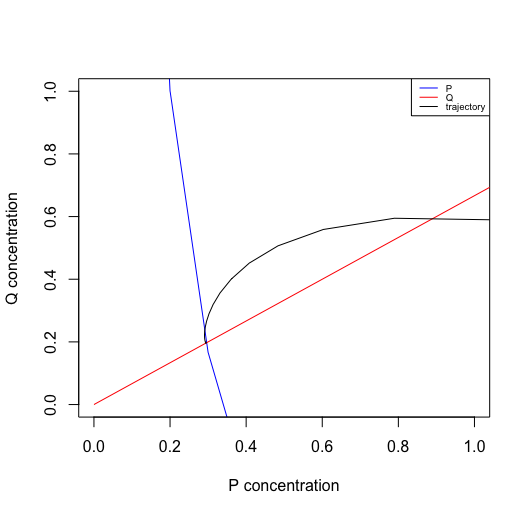
\includegraphics[width=\textwidth]{images/2e.png}

\end{document}
